\part{新古典经济思想及其批判}

19世纪70年代早期,来自三个不同国家、拥有三种不同背景的三位经济学家分别独立地提出:一
件商品的价值或者价格,取决于商品对消费者的边际效用。1871年,威廉·斯坦利·杰文斯用
英语出版了他的《政治经济学理论》,卡尔·门格尔用德语出版了他的《国民经济学原理》。
三年之后,在瑞士教书的法国经济学家莱昂·瓦尔拉斯用法语出版了他的《纯粹政治经济学纲
要》。这些经济学家的重要贡献——以及阿尔费雷德·马歇尔,他在19世纪60年代后期就形成
了这些观点,但直到1890年才将它们发表——在经济理论中运用了边际分析。他们的工作
是后来被称之为新古典经济思想的开始。

到了19世纪90年代,很多经济学家认识到这一工具能够被用于分析收入分配的决定力量,他
们发展了边际要素生产力概念。这一时期边际分析的增加,引起人们将注意力几乎专门放在
微观经济理论问题上。这样,从1870年至1930年正统经济理论或者说新古典经济理论在很大
程度上忽视了宏观经济问题,即收入水平及其增长速度的决定力量。在微观经济理论范围内,
新的分析主要被用于如下情形,即竞争性市场在可替代的用途之间配置稀缺资源。边际分析
在方法上基本上是演绎的,使用了高度抽象的家庭与厂商模型,家庭与厂商被假定为试图使
效用和利润最大化。这些抽象模型的发展,引起了关于方法论的争议,我们将对此予以考察。

尽管杰文斯、门格尔、瓦尔拉斯对于边际分析的出现来说都是重要的,然而,杰文斯和门格
尔集中于边际分析的应用。杰文斯是在家庭层面上进行研究,门格尔是在家庭与厂商两个层
面上进行研究。对瓦尔拉斯来说,边际分析的应用仅仅是阐明一般均衡模型的一种手段。杰
文斯和门格尔寻找因果关系的简单线路;瓦尔拉斯看到了所有经济变量的相关性。马歇尔在他
的局部均衡系统中,使用边际分析作为一个建筑构件,并且也看到了所有价格和所有经济活动
的相关性。正是瓦尔拉斯和马歇尔理论上较强的复杂性,使他们对后来的经济思想产生了深远
的影响。

瓦尔拉斯的工作与马歇尔的工作的区别在于,瓦尔拉斯的分析是以这样一种方式组织的,即
同时分析所有的市场——一种一般均衡,,而不是一种局部均衡。方法上的差别代表了关于经
济学目的的不同方法论观点。马歇尔把经济学视为分析的发动机,以考虑真实世界的问题。
他认识到了一般均衡问题,但是,他认为它们应当保留在人们的内心中,需要的时候再调出
来。瓦尔拉斯较多地关注理论结构的正式逻辑,较少关注将其用于真实世界的政策问题。

马歇尔与瓦尔拉斯都有资格作为新古典经济学之父,新古典经济学将价格看成是由供给与需
求两者决定的,并且认识到所有经济活动的复杂相关性。价格的双重决定以及意识到所有变
量的互相依赖,标志着古典劳动价值理论、古典生产成本价值理论以及古典收入分配剩余理
论的终结。

因为新古典分析的形成实际上是一系列稍微不相关的发展的一部分,所以,我们把
对1870——1900年期间的论述分为几章。第8章考察边际分析的一些先驱者和经济学家杰文斯、
门格尔以及瓦尔拉斯,19世纪70年代早期他们将边际分析大量用于需求理论。第9章研究了边
际分析在生产理论中的应用,和由此产生的边际生产力概念,以及紧跟着对资本和利息理论
的贡献。接下来的两章展现了两个人的贡献,他们铸就了完整的市场理论。其中,第10章探讨
了阿尔弗雷德·马歇尔的经济学,他形成了当前局部均衡分析或供求分析的基本框架,并试图
解决这一时期提出的很多理论和方法问题。第11章考察了1874年首次由菜昂·瓦尔拉斯提出的
一般均衡模型。

在最后两章中,我们将讨论对新古典经济学的一些主要批评,这些主张对于现代经济学的塑造
是重要的。在第12章中,我们考察对新古典经济学的一些早期批判,即德国历史学派和美国制
度主义。在第13章中,我们将回顾奥地利经济学家和其他经济学家,他们考察了社会主义经济
的理论基础。我们将在第17章中转向非正统经济学家,考察几个现代非正统群体,在经济思
想的演进中,他们仍然扮演着一定的角色。

\chapter{杰文斯、门格尔以及边际分析的基础}

19世纪最后三十年见证了新古典微观经济理论的诞生。在这一时期,一套新的分析工具的建
立,促使古典经济学向新古典经济学转变。其中最为重要的分析工具是边际分析,它开始使
数学在经济分析中的运用显著增加。然而,对边际分析的认可以及对其重要性和含义的充分
认识,不是一夜之间发生的;它们在1870年至1900年期间缓慢地发展。边际分析首次值得注意
的应用是在需求定理中。19世纪70年代早期,三位学者独立地将边际分析应用于需求定理,
形成了边际效用的概念。其中的两位——瓦尔拉斯和门格尔也将边际分析应用于厂商理论中。
瓦尔拉斯甚至超越了边际分析的应用,阐述了一般均衡分析,我们将在第11章中涉及这个问题。

边际主义者一致认为,经济学通常关注资源配置或者微观经济学,但是,就所应用的适当方法
来说,他们有不同的看法:杰文斯提倡更多的经验研究;门格尔主张抽象演绎逻辑,瓦尔拉斯
则提倡数学方法。

这三位伟大的边际主义者对后来经济思想的发展产生了深远的影响,我们将对此做出评价并
结束本章内容。

\section{历史链接}

早期古典学者(以亚当斯密为例)提供了一个明显的对比。他们主要对分析经济发展过程、发
现并实行能够产生较高经济增长率的政策感兴趣。斯密是一位以关联性政策为导向的发展型
的宏观经济学家,他很少对抽象的经济理论感兴趣。他的方法反映出他在人文学科和社会科
学方面受到的广泛训练,是理论与历史描述的一种松散结合,不同于未来更加数学化的方
法。

19世纪早期,李嘉图转变了经济学的范围和方法。首先,他由关联性的分析转变为比较抽象
的演绎分析,强调抽象模型中内在逻辑一致性的重要性。他这么做,为新古典经济学提供了
方法上的依据。其次,李嘉图认为,经济学不应当集中在发展问题上,而应当主要集中研究不
同时期决定收入功能性分配的力量。这使得他去考察当时为人所知的价值理论或者价格理论,
也就是现在所知的微观经济理论。在分析不同时期收入分配的决定力量时,李嘉图在其地租
理论中开始运用边际分析,其地租理论后来成为微观经济理论的一个主要组成部分。

在紧随李嘉图之后的时期,经济理论与资本主义制度本身受到人道主义者和社会主义者的许
多批评。尽管这些批评对经济理论的技术性内容没有什么影响,但是,它们的确质疑了自由
放任是一种理想的政府政策的古典假设,并引发了变革,这些变革进一步使这一专业
对1870年至1900年之间的发展有所准备。随着经济学变得更加专业化,经济学家开始仔细察
看古典理论的技术性内容,尤其是劳动价值理论。在约输·斯图亚特·穆勒和拿骚·西尼尔的掌
控下,古典经济学采用了生产成本价值理论,既包含资本成本,也包含劳动成本。

李嘉图的理论与英国经济实际运行之间越来越多的矛盾,也为这一时期的发展做出了贡献。
特别是,人口增加与大多数人实际收入上升同时发生。因此,经验证据反驶了马尔萨斯的人
口学说,但是,当时的经济学家仍然坚持它是古典体系的基本假定。当穆勒在1869年最终从对
工资基金学说的忠诚中退出时,古典体系的衰落就几乎完成了。那时,李嘉图体系中的三个
基本工具和假设——劳动价值理论、马尔萨斯人口学说、工资基金学说——事实上已经被放
弃了。1874年,在《政治经济学若干基本原理》中,J.E·加尼斯(J.E.Caimes,1823--1875)试
图挽救古典体系,但是没有什么效果。

\subsection{边际分析的先驱者}

古典经济学并不是在一夜之间变成新古典经济学的;观点与理论结构的重塑是逐渐发生的。
例如,效用的观点在经济文献中已经存在很长时间。大约两千年前,亚里士多德就运用了使
用价值的概念,18世纪后半部分,杰里米·边沁也在功利主义哲学中使用了效用的概念。

19世纪,一群二流经济学家对如下原理已经拥有清晰的概念,即随着消费产品数量的增加,产
品将给消费者带来递减的边际效用。然而,这些经济学家中没有一个人能够详细而充分地阐
述边际效用递减的概念,或者将它用于解决经济问题。回顾往事,凭借几近完美的后见之明,
我们能看到,边际分析最早是在1834年出现的,当时,塞缪尔·蒙迪福特·兰格菲尔
德(SamuelMountifortLongfield,1802——1884)在《政治经济学讲义》中因不满于劳动价值理
论,发展了一种边际生产力理论。W.F·劳埃德(W.F.Lloyd)……朱尔斯·杜皮特(Jules
Dupuit)……、赫尔曼·海因里希·戈森……理查德·詹宁斯……尽管安东尼·奥古斯丁·古诺在
他的《财富理论之数学原理的研究》一书中没有呈现效用理论,但是,在运用边际工具来发
展相当透彻的厂商经济学分析方面,他是最早的且对以后有巨大影响的一位思想家。他能够
界定需求,确定在较低价格上需求的数量将会增加。

另一位重要的经济学家是约翰·海因里希·冯·杜能(Johann Heinrich von Thünen
1783--1850)。约瑟夫·熊彼特将杜能描述为是一位在他自己所处的时代之前进行创作的经济
学家。在共同以《孤立国》为名出版的几部书中,冯·杜能通过微积分学来运用边际分析,他
认识到了工资的边际生产力理论、收益递减规律以及地租方面的一些重要见解。他和古诺是
最早的数理经济学家。这些经济学家中的一些人,后来被发现是“被忽视了的经济学家”,
但是另一些人,尤其是古诺和冯·杜能(阿尔弗雷德·马歇尔对他们产生的影响表示感谢)对后
来的经济理论做出了显著贡献。

乔治,斯蒂格勒就效用理论的发展进行创作时观察到:

\begin{quotation}
  效用生产手段(例如收入或者面包)的等量增加,引起效用增量的递减,这个原理是一件平凡
  的事情。对这件平凡事情的陈述,最早出版时是偶然的;它在经济学的发展中并不具有重要性,
  并没有授予其作者智力名望。只有当这一陈述在逻辑上得到发展,或者明确地用于经济问题
  时,它才获得了关注,并且只有当相当多的经济学家被说服,将它融入到他们的分析中时,它才获得了
  重要性。关注与重要性当然是程度问题。
\end{quotation}

由遵循斯蒂格勒的说法,当我们确定集中考察哪些经济学家时,我们的标准是他们对后来经济
思想和政策的影响。

\section{杰文斯、门格尔以及瓦尔拉斯}

在1871年至1874年期闻,杰文斯、门格尔以及瓦尔拉斯出版了对正统经济理论产生影响
的书。他们的影响虽然不是直接的,但却在19世纪最后的二十五年中发展着,他们的后继者即
边际效用的第二代理论家,为一些“新”观点而战,并逐渐获得了认同。杰文斯、门格尔以
及瓦尔拉斯关于最终产品价值或价格决定力量的观点十分相似,所以我们通过主题来考察他
们,而不是分别对他们进行论述。

在这些边际分析发展者之间,存在一些非常重要的差别,在本章后半部分我们将予以研究。
尤其是就经济学的适当方法而言,他们有不同的看法。门格尔应当受到特别的关注,原因是
现代奥地利学派声称门格尔是他们的智力来源。然而,瓦尔拉斯的一般均衡分析,以及他将
边际概念与一般均衡理论的结合,也因为它们后来在现代微观经济理论中的重要性而显得独
一无二。他们的贡献足以重要到完全有理由单独开设一章。

\subsection{这是理论上的一次革命吗}

这三位相互独立工作的经济学家确信,他们发展了一种独特的革命性
分析,用来解释决定相对价格的力量。杰文斯最为简洁地陈述了这一点:
\begin{quotation}
  不断的思考和研究使我得出有些新奇的观点,即价值完全取决于效用。流行的观点认为劳
  动是价值的起源,而不是效用;有些人其至明确地声称劳动是价值的原因。
\end{quotation}

门格尔的陈述从个人角度看比较谦逊,虽然有些民族主义:
\begin{quotation}
  对我来说,特别高兴的事情是,这里所论述的领域,由我们学科中最一般的原理组成,真
  实地说,它丝毫不是德国政治经济学近来发展的产物;这里所试图从事的是对我们学科中最
  重要原理的改革,因此是建立在以前工作所设置的基础之上,那些工作几乎完全是由于德
  国学者的勤奋所致,
\end{quotation}

瓦尔拉斯因其一般均衡分析而者称,他也相信其贡献的原创性和独
特性:
\begin{quotation}
  现在我能够开始出版一部关于政治经济和社会经济要素的著述,且确信这是一个新的计划,
  并按照一种原创性的方法来详细阐述。我斗胆地说,我所得出的结论在几个方面不同于当
  前的经济科学。
\end{quotation}

杰文斯对经济理论的贡献主要是将边际分析用于需求。门格尔的贡献是将边际分析用于需求
与供给,虽然对供给注意不多。瓦尔拉斯的贡献是将边际分析用于需求与供给,他也对供给
注意不多,并且他的贡献还在于阐明了经济体的一般均衡模型。是的,他们是原创性的,因为
他们的观点在某种程度上影响了经济理论后来的发展,以前运用边际分析的经济学家们的观
点,并不具备这种影响(例如,戈森和古诺)。但是,他们的工作在什么程度上是革命性的,
只能通过比较他们的观点和以前的古典理论,以及依靠新古典微观经济理论后来的发展来决
定。

\subsection{古典价值理论的不充分}

三位经济学家都发现,对于解释价格的决定力量来说,古典价值理论是不充分的。其中主要的
批评是生产成本价值理论缺乏一般性,其原因在于很多产品的价格不能在古典框架中加以分
析。他们批评李嘉图的劳动价值理论,以及西尼尔和穆勒的生产成本理论,因为那些理论需
要对具有固定供给的产品价格进行单独的解释。具有完全无弹性(垂直的)供给曲线的产品价
值或者价格——例如,土地、稀有古币、绘画或者酒——并不取决于它们的生产成本。生产
成本价值理论的问题还在于,它认为一件产品的价格或者价值,来自于过去发生的成本。杰
文斯、门格尔以及瓦尔拉斯都认为,产品生产中发生的大量成本,不一定导致高价格。按照
边际效用理论的观点,价值取决于效用或者消费,不是来自于过去,而是来自于未来。无论在
产品生产中发生了什么成本,当产品到达市场时,其价格将取决于购买者预期获得的效用。
错误地预见对其产品需求的生产者,痛苦地明白这一点。呆滞商品(dead stock)这一术语用
来指需求下降从而使价格低于生产成本的产品。杰文斯辛辣地表达了这一点:“事实是,曾经
支出的劳动对任何商品的未来价值都没有影响,它永远离开并失去了。在商业中,过去的事
永远都是过去的事。”

因此,这三位经济学家致力研究的问题是:价值是因最终产品中的生产要素而产生(就像古典
价值理论所主张的那样),还是最终产品决定了生产要素的价值。边际效用学派断言,生产要
素是有价值的,但是其价值的范围是由消费这些要素所生产的最终产品获得的边际效用决定
的。然而,生产要素或者说中间产品,并不在最终产品上赋予价值。理查德·维特利是李嘉图
劳动价值理论的一位早期批评家,他在19世纪30年代非常巧妙地提出了这一观点,当时他说,
因为人们都忙于搜寻珍珠,所以珍珠不贵重;但是,因为珍珠贵重,所以人们都忙于搜寻珍
珠。

根据边际效用经济学家的观点,前古典与古典经济理论的另一个基本缺陷是,它们未能认识
到,价格决定中的重要因素不是总效用或平均效用,而是边际效用。亚当·斯密从较早的文献
中挖据出了古老的“钻石——水悖论”:钻石具有和较高的价格但较低的效用,水具有较低的
价格但较高的效用。古典理论家不能说明这一悖论,原因在于,他们根据钻石和水带给消费
者的总效用来思考这个问题,并不了解边际效用的重要性。\cref{tab:mengeer}模仿门格尔使用过的表
格,很容易地举例说明了这个悖论。

% Please add the following required packages to your document preamble:
% \usepackage{booktabs}
% \usepackage{graphicx}
\begin{table}[htbp]
  \centering
  \caption{门格尔的表格(各商品种类的边际效用)}
  \label{tab:mengeer}
  \begin{tabular}{@{}c|*{10}{c}@{}}
    \toprule
    被消费单位 &\Rnum{1}& \Rnum{2} & \Rnum{3} & \Rnum{4} & \Rnum{5} &
                                                                      \Rnum{6}& \Rnum{7} & \Rnum{8} & \Rnum{9} & \Rnum{10} \\ \midrule
    1 &10 & 9 & 8 & 7 & 6 & 5 & 4 & 3 & 2 & 1 \\
    2 &9 & 8 & 7 & 6 & 5 & 4 & 3 & 2 & 1 & 0\\
    3 &8 & 7 & 6 & 5 & 4 & 3 & 2 & 1 & 0 \\
    4 &7 & 6 & 5 & 4 & 3 & 2 & 1 & 0 \\
    5 &6 & 5 & 4 & 3 & 2 & 1 & 0 \\
    6 &5 & 4 & 3 & 2 & 1 & 0 \\
    7 &4 & 3 & 2 & 1 & 0 \\
    8 &3 & 2 & 1 & 0 \\
    9 &2 & 1 & 0 \\
    10 &1 & 0 \\
    11 &0 \\ \bottomrule
  \end{tabular}%
\end{table}


随着更多的商品被消费,商品的边际效用递减。假设第I种产品是水,第II种产品是钻石。如果消费
者已经消费了8单位的水,没有消费钻石,那么,下一单位水的边际效用将只有2,但是,第一
单位钻石的边际效用将是3。水的总效用是其边际效用的总和,显然大于钻石的总效用,然而,
另一单位钻石的价值高于另一单位水的价值。按照边际效用经济学家的观点,古典经济学家
未能认识到这一原理在解释价格中的重要性,这正是为什么他们没有能力发展一种正确的价
格理论的主要原因之一。钻石的价格高于水的价格,原因在于,正是边际效用决定了消费者的
选择,从而决定了价格。

\subsection{什么是效用}

边际效用经济学家遵循了正统古典经济理论的如下假定,即个人是理性的和精于计算的。消
费者或家庭在作购买决策时,考虑他们预期从产品消费中享受到的边际效用。这就引起了两
个问题什么是效用,以及它是怎样度量的?杰文斯、门格尔、瓦尔拉斯解决这些问题的方法几
乎是相同的:他们根本不直接回答这些问题。没有人使用边际效用(marginal utility)这一术
语;门格尔甚至不用效用(utility)这一词,而宁可说“满足的重要性”。三个人都假设存在
效用,并且个人的内省将发现不同最终产品的不同效用。对他们来说,效用显然是一种没有
明确度量单位的心理现象。是用线性空间(如一英寸),还是体积(如一夸特),抑或重量(如一
盎司)来度量效用?他们认为,效用是最终产品或者消费者产品的一个特征,但是,生产要素和
只能间接消费的产品怎样呢?我们应当怎样度量不是为了消费,而是为了与其他商品交换而获
得的产品的效用呢?门格尔比杰文斯或瓦尔拉斯更加关注最后这个问题。这些产品从它们最终
交换来的产品消费中获得效用,杰文斯将这种产品的效用称为“获得的效用”。

因此,杰文斯、门格尔还有瓦尔拉斯,并没有清楚地解释效用概念的性质,他们假定了现在
为人所知的边际效用递减(diminishing marginal utility)原理,声称随着一件产品的消费
增加,其边际效用减少。这是基于无论边际效用是什么,它都能够被度量这一假设。门格尔
和瓦尔拉斯没有论述可度量性。杰文斯说尽管我们现在没有能力度量效用,但是,进一步的发
展会在将来实现这种度量。然而,从他们著作中所给的例子来看,显然,三个人都假定了效
用最重要的可度量性。

作为一个初步估计值,杰文斯和瓦尔拉斯利用效用函数的数学表达,假设所消费产品的数量
和效用的数量能够连续分割。两个人都认识到这一假设的非现实性,并在他们的表达中人允
许不可分性的存在,这导致了不连续的函数。因为门格尔的方法只是运用了算术表格,所以,他
的所有函数都是不连续的。绘图时连续函数具有平滑的曲线,而不连续的函数具有台阶状的
曲线。这一点具有较小的理论意义。例如,戈森第二定律断言,消费者将通过购买来使其总
效用最大,所以,花在一种产品上最后一单位的货币,与花在任何其它产品上的最后一单位货
币相比,提供了相同的边际效用。这一效用最大化(utility maximization)命题的代数表达是:
\begin{equation}\label{eq:second}
  \frac{MU_A}{P_A} = \frac{MU_B}{P_B} = \frac{MU_C}{P_C}
\end{equation}

如果效用函数是连续的(具有平滑的曲线),那么,即使发生数量与效用的微小变动,也能
使等式得到满足。但是,如果效用函数是不连续的,那么,在等式不被满足的情况下,消费
者也可能实现了最大化。

\subsection{效用的比较}

假定效用能够被度量,这又会引起为外一系列问题。三位经济学家都假定个人有能力对不同
商品的效用进行比较,而没有去检验这个问题。因此,另一杯啤酒的边际效用就能与另一双
鞋的边际效用进行比较。一个更重要的问题涉及人与人之间的效用比较(interpersonal
comparisons of utility):一个人从消费另一杯啤酒中获得的效用,有可能与另一个人从消
费另一双鞋子或另一杯啤酒中获得的效用进行比较吗?门格尔与瓦尔拉斯从未涉及过这样的问
题,然而,他们的分析并不依赖于人与人之间的效用比较是可能的这一假设。杰文斯认为,
这种比较是不可能的,但是(按照其作品的典型方式)他还是进行了这种比较。

我们将在后面返回到人与人的效用比较上,原因在于,它们对于某些公共政策和福利经济学
的问题来说,还是有意义的。在此期间,简单地看一个杰文斯的例子将会有所帮助。杰文斯
认为,给收入高的人一个额外的收入量,与给收入低的人同样的收入量相比,将会产生较低
的边际效用。这就假定了人与人之间的效用比较是可能的。杰文斯只是提出可以进行人与人
之间的效用比较。

如果我们假设人与人之间的效用比较是可能的,并且每个人拥有相同的收入效用函数(例如,
收入的第999美元的边际效用,对每个人来说都是相同的),那么考虑到这两个假设,收入的
一种理想分配(即社会总效用最大的分配)将是收入的平均分配。从\cref{fig:hood1}中能够看出这一结
论。

\begin{figure}[ht]
  \centering
  \subcaptionbox{\label{fig:hood1}罗宾·胡德效应 }{%
    \begin{tikzpicture}[scale=0.8]
      \draw (0,0) node[below left] {$O$};
      \draw[very thick] (0,5) -- node[left=10pt, text width =1em] {收入的边际效用} ++(0,-5)  -- node[below=10pt] {收入} ++ (7,0);
      \draw[dashed] (2,0) node[below]{$P$} -- (2,2.2) node[above]{$B$};
      \draw[dashed] (4,0) node[below]{$R$} -- (4,1.8) node[above]{$A$};
      \path (2,2.2) -- (4,1.8) coordinate[pos=-0.6](dd) coordinate[pos=2](ff);
      \draw (dd) node[left]{$I$} --(ff) node[right]{$I'$};
    \end{tikzpicture}%
  }\hfill
  \subcaptionbox{\label{fig:hood2}相反的罗宾·胡德效应}{%
    \begin{tikzpicture}[scale=0.8]
      \draw (0,0) node[below left] {$O$};
      \draw[very thick] (0,5) -- node[left=10pt, text width =1em] {收入的边际效用} ++(0,-5)  -- node[below=10pt] {收入} ++ (7,0);
      \draw[dashed] (2,0) node[below]{$P$} -- (2,2.2) node[above]{$B$};
      \draw[dashed] (4,0) node[below]{$R$} -- (4,2.8) node[above] {$A$};
      \path (2,2.2) -- (4,1.8) coordinate[pos=-0.6](dd) coordinate[pos=2](ff);
      \draw (dd) node[left]{$p$} --(ff) node[right]{$p'$};
      \coordinate (ff2) at ([yshift=1cm] ff);
      \coordinate (dd2) at ([yshift=1cm] dd);
      \draw (dd2) node[left]{$r$} -- (ff2) node[right]{$r'$};
    \end{tikzpicture}%
  }
  \caption{穷人与富人收入的边际效用比较}
  \label{fig:hood}
\end{figure}

两个假设使我们能够用一条曲线$II'$来表示富裕者和贫穷者收入的边际效用函数。(暗含的
第三个假设是边际效用递减原理也运用于收入。)假定富裕者的收入为$OR$,贫穷者的收入
为$OP$。向富裕者征收的一美元税,使其总效用减少了$RA$,如果这一美元给了贫穷者,将使
其总效用增加$PB$。收入从富裕者向贫穷者的转移,增加了社会总效用,原因在于$PB>RA$。
此外,如果重复这一过程,社会总效用将增加,直至富裕者与贫穷者的收入相等为省。

假定我们改变了其中一个假设,假设个人具有不同的收入效用函数,并且高收入者收入的边际
效用函数位于低收入者的上方。这一模型用\cref{fig:hood2}表示。曲线$rr'$表示富裕者收
入的边际效用递减,曲线$pp'$表示贫穷者收入的边际效用。两条曲线的相对位置表明,富裕
者比贫穷者能够从既定的收入量中获得更多的边际效用。通过拿走贫穷者的收入给富裕者,
将实现社会总效用最大的理想的收入分配,原因是$RA>PB$。可以将其称为相反的罗宾·胡德
效应。显然,初始收入分配不同,或者曲线$pp'和rr'$的位置不同,将会导致不同的结
论。

无论杰文斯、门格尔还是瓦尔拉斯,都没有对收入分配的含义进行研究,原因在于,他们认
为——杰文斯明确地,门格尔和瓦尔拉斯含蓄地——表示人与人之间的效用比较是不可能的。

\subsection{效用函数}

尽管杰文斯、门格尔、瓦尔拉斯没有清楚地考察效用函数的准确形式和性质,但杰文
斯和瓦尔拉斯还是写出了将总效用与所消费的产品数量相联系的等式,并且门格尔的语言和
算术例子也表明,他的总效用函数概念与杰文斯和瓦尔拉斯的概念是相同的。按照这些经济
学家的观点,个人从消费一件产品中所获得的效用,唯一地取决于其所消费的那种产品的数量。
它并不取决于所消费的其它产品的数量。总效用函数,即从消费所有产品中获得的效用,因此就是一种加法函
数,杰文斯和瓦尔拉斯用下列形式来表示:
\[总效用=f^1(Q_a)+f^2(Q_b)+f^3(Q_c)+ \cdots\]

这表明总效用它否定了产品之交互补或替代关系的存在。但在现代微观经济理论中,这些互补
和替代关系并没有被否定,总效用函数被写成了更一般的形式,例如:
\[总效用=f(Q_a,Q_b,Q_c\cdots)\]

\subsection{效用、需求以及交换}

使杰文斯、门格尔、瓦尔拉斯与他们的前辈(除了戈森之外)相区列
的是,他们不仅假定了边际效用递减原理,而且试图确定消费者效用最大
化的条件。并形成一种交换理论。杰文斯和瓦尔拉斯由于对效用与需求之
间关系的研究而相当有名。瓦尔拉斯由于数学能力较强,在这些研究方面
他是三个人中最成功的。尽管他不太关注边际效用递减的概念,但是,他
对经济体不同部门的相关性有更成熟的理解。

戈森第二定律表明,消费者通过如下方式支出有限的收入能使效用最
大化,即花在任何一种特定产品上的最后一单位货币所产生的边际效用,
与花在任何其他产品上的最后一单位货币所产生的边际效用相等。

尽管门格尔和杰文斯确立了这一假设的精髓(门格尔做了语言上的解释,以及粗略的算术举
例,杰文斯运用了比较成熟的数学符号),留给瓦尔拉斯的正是在他著名的《纯粹政治经济学
纲要》第8讲中,从数学上得出消费者效用最大化时成立的等式。

如果个别消费者效用是解释个人和市场需求的根本力量,那么,就有必要表明效用函数与需求
曲线之间的关系。门格尔没有对这一过程进行尝试,没有直接在语言上、图形上或者算术上
涉及需求曲线。杰文斯在其分析中使用了需求函数,但是未能确立效用与需求之间的关系。瓦
尔拉斯能够确立效用与需求之间的关系,并表明需求背后的根本力量是边际效用。

三位先驱者都试图说明边际效用、消费者满足最大化以及产品交换之
间在市场上的关系。门格尔是最不成功的。杰文斯能够说明两种产品、两
个个体的简单市场上的这些关系。如果个体G拥有谷物,个体H拥有牛肉,
他们以物易物,那么,均衡的最终位置能被简明地表述为:“任何两种商品
的交换比率,在交换完成之后,将是可供消费的商品数量的最后效用程度
比率的倒数”。杰文斯的陈述能被转换成下面的等式:
\[ \frac{谷物对G的MU}{牛肉对G的MU} = \frac{谷物对H的MU}{牛肉对H的MU} = \frac{交
    易的牛肉数量}{交易的谷物数量} = \frac{谷物的价格}{牛肉的价格} \]

与杰文斯或门格尔相比,瓦尔拉斯以一种更加彻底和一般性的方式表明了边际效用、消费者
满足最大化以及交换之间的关系。

\subsection{生产要素的价值}

古典价值理论主张相对价格取决于生产成本,强调效用的早期经济学家对此予以批评。他们
说这意味着价值来自于过去;他们的观点与之相反,认为价值来自于未来,来自于消费最终产
品时所享受到的预期效用。这些边际效用经济学家怎样解释生产要素的价格呢?关于这个问题,
杰文斯和门格尔一方与瓦尔拉斯另一方之间存在重大区别。

杰文斯和门格尔两人都讨论了这个问题,尽管门格尔的处理比杰文斯更加完全,然而,两个
人实质上取得了相同的结论。他们认为,价值的因果关系不是从生产成本到最终价格,而是相
反的方向,因而他们提出生产要素不是决定价格的因素(price-determining),而是被价格
决定的(price-determined)。一件最终产品的价格取决于其边际效用,生产要素(另外也称
为中间产品或较高次序的产品)的价格取决于所生产的最终产品的效用。因此,杰文斯和门格
尔在局部均衡的框架中处理最终产品和生产要素之间的因果关系。因为瓦尔拉斯在其一般均
衡分析中阐明了对价值的考虑,所以,他比杰文斯或门格尔更充分地了解这个问题,并且把因
果关系看得更加复杂。

\subsection{对杰文斯和门格尔的评价}

通过比较杰文斯和门格尔的价值理论与约翰·斯图亚特·穆勒的价值理论,我们能够看到,杰
文斯和门格尔对古典价值理论的批评,在很多方面是不正确和不充分的。正如我们
在\cref{cha:mill}和在\cref{fig:mulema}中看到的那样,穆勒设想了价值的三种可能情形,
完全无弹性的(垂直的)供给曲线;制造业的完全有弹性的(水平的)供给曲线,穆勒假定制
造业由成本不变的行业组成;以及代表农业的向上倾斜的供给曲线,穆勒假定农业是成本递增
的行业。穆勒断定,在成本不变的行业中,生产成本单独决定价格。杰文斯和门格尔没能反
驶这一点。

对于供给固定从而拥有完全无弹性(垂直的)供给曲线的商品来说,穆勒认为供给与需求决定
了价格。杰文斯与门格尔也没能反驳这个假设。他们的说法是在供给既定的情况下,需求决定
价格。他们很可能同样有理由说,在需求既定的情况下,供给决定价格。杰文斯和门格尔没
有分析穆勒成本递增行业向上倾斜的供给曲线,原因在于,他们总是假设成本是既定的。这并
不意味着穆勒的价值理论没有缺点,但是,它的确表明杰文其和门格尔没能支持他们自己的
所有主张。

门格尔简洁地陈述了他对古典价值理论的批评:“在我们学科以前的发展中,最惊人的具有最
深远后果的基本错误之一,是认为因为产品在对我们来说有价值的生产中被使用了,所以产
品为我们获得价值。”门格尔断言,恰恰是效用而不是生产成本决定了价值。“产品的价值起
因于它们与我们的需要有关联,它不是内在于产品本身中的。”因为杰文斯的陈述更激烈,
所以,他显得稍微敏感些:“反复的思考与研究,使我得到一种颇有几分新奇的意见。即价值完全取决于
效用。”

杰文斯和门格尔使用的例子却表明,价值或者价格并不完全取决于效用或需求,而是取决于供
给与需求两者。尽管这些经济学家和他们的弟子宣称,价值唯一地取决于效用,然而,他们
自己的分析否定了这一假设。在这点上杰文斯是最好的例子。他的《政治经济学理论》第二
段以我们刚才引用过的句子作为开头。在做了这一强烈的表述之后,杰文斯接下来的四句话
反驳了他自己。

\begin{quotation}
  流行的观点认为价值的起源是劳动,而不是效用,甚至有人断言说劳动是价值的原因。反
  之,我却要说明,我们只需细心探索出效用变化——取决于我们所拥有的商品量——的自然法
  则,关于交换,即可得到满意的理论。普通的供求律是这个理论的一个必然的结果罢了。这
  一理论是和事实调和的;即令表面上相信劳动是价值原因的理由,这种理由亦不是不能解释。
  劳动常决定价值,但只间接地决定价值;那边是增加或限制供给,以变化商品的效用程度。
  (郭大力译《政治经济学理论》1984版,29页)
\end{quotation}


杰文斯进一步摧毁了(1)他所认为的价值完全取决于效用的主张,(2)他在《政治经济学理论》
第4章中所声称的对古典价值理论的反驳形成了他的交换理论。在此,他正确地表明,假定两
种产品的固定供给为两个个体所持有,那么这些产品的价格与所交换的数量,将取决于两种
产品对两个个体的边际效用。尽管这一假设在形式上是正确的,然而,它没有包括供给不是
固定的而是变动的这种通常的经济状态。当杰文斯不再讨论供给固定的假设,开始分析成本、
供给、边际效用以及价格之间的关系时,他得出了下面的因果关系,

\begin{quotation}
  \noindent 生产成本决定供给;\\
  供给决定最后的效用程度;\\
  最后的效用程度决定价值。(同上,131页)
\end{quotation}

可以依据若干理由来批评这一假设。首先,杰文斯没有提供成本或供给理论。此外,该假设
认为一连串的因果关系是从生产成本到价值或者价格。如果这样的一连串因果关系的确存在,
那么将有可能忽略这一连串的中间部分,得出生产成本决定价值的结论。

杰文斯和门格尔的错误在于,他们试图寻找边际效用与价格之间简单的单行道的因果关系。
他们没有觉察到成本、供给、需求以及价格是彼此相互依赖、相互决定的。

\subsection{古典价值理论与新兴的新古典价值的比较}

在穆勒的第一种情形中\cref{fig:mulea},当供给完全没有弹性(垂直的)时,古典生产成本
价值理论没有充分解释价格的决定力量。在这些情况下,价格取决于供给与需求,生产成本
可能对供给没有影响。但是,价格只取决于需求的“杰文斯-门格尔”观点也不能令人满意,
原因在于,穆勒这时假定供给是固定的。穆勒在第一种情形中所给出的几个例子解释了这一
点。假定供给仅存一张的错版邮票,价格将由需求水平来确定。价格取决于供给和需求两者
的观点,能通过假定发现了十枚这样的邮票来得到证明:在这种情况下,供给曲线将向右移
动,价格将会下降。第二个例子,一天天腐烂下去的食品店水果,食品店将降低价格来获得
任何需求,因为得到一些收入要好于商品腐烂。第三个例子,供给固定,但是被“生产者-销
售者”以某一价格持有的制造业产品。这样的一种价格通常被称为“保留价格”,可以由生
产者根据生产成本适当地加以确定。在这个例子中,供给曲线看上去像相反的字母L,水平部
分代表成本水平,垂直部分代表产品现有的总库存。

在穆勒的第二种情形中\cref{fig:muleb},供给完全有弹性(水平的)且存在不变成本,价格
完全取决于生产成本。此时,穆勒所代表的古典价值理论完全正确,“杰文斯-门格尔”观点
完全无效。

正如面对第一种情形一样,,“杰文斯-门格尔”和古典理论两者都未能解释穆勒的第三种情
形中价格的决定\cref{fig:mulec},在这种情形中,供给曲线向上倾斜(成本道增的特点所
在)。在这些情况下,穆勒断定,价格取决于最不利条件下的生产成本。用现代术语来说,价
格取决于最后生产的产品的边际成本。在既定需求下,生产成本或者供给决定价格。杰文斯
和门格尔断定价格取决于边际效用:在既定供给下,需求决定价格。因为价格既然取决于供
给与需求两者,所以双方的观点都是错误的。此外,杰文斯和门格尔与古典学者都犯了同样
的错误,即试图寻找简单的因果链条来解释价格:古典的因果关系是从生产成本到价格,而
杰文斯--门格尔的因果关系是从效用到价格。他们都未能看到这些变量是相互依赖的,并且
相互决定彼此的价值。就像我们将在第10章和第11章中看到的那样,马歇尔与瓦尔拉斯的非
凡才智使他们领会了这种相互依赖。

杰文斯和门格尔在他们对边际分析的说明中存在一些问题和欠缺;后来的经济学家认识到了
这些问题和欠缺,并予以改善。例如,杰文斯只解决了一部分最大化难题,仅将其注意力限
制在消费者一方。门格尔注意并解决了难题的两个方面:家庭与厂商。三位边际主义的创始
人中,没有一位从最终产品市场深入到要素市场,并形成边际生产力分析的概念与含义。这
些进步意义重大,足以在第9章中引起特别的注意。

杰文斯和瓦尔拉斯没有直接的追随者来“整理”他们对边际分析的首次接触。门格尔则比较
幸运,他有两个学生,他们立刻开始从事效用和边际主义事业,接下来我们考察他们对经济
思想潮流的贡献。

\section{第二代奥地利学者}

\subsection{弗里德里希·冯·维色}

当门格尔1871年出版他的《原理》时,维色(Friedrich von Wieser,1851--1926)年方二十。
他同欧根.冯,庞巴维克(Eugen von Bohm--Bawerk,1851--1914)一起,都是门格尔的学生,
维色于1903年在维也纳大学接替了门格尔的职位。庞巴维克也在那所大学教书。而且他们也
有自己的学生:路德维格-汉:米塞斯(Ludwig von Mises,1881--1973)和约瑟夫熊彼特。米
塞斯还培养了一大批新一代的经济学家。由于受门格尔及维也纳大学的影响,使思想史学家
们不得不谈及奥地利学派(Austrianschool),我们将在本章和后面的一些章节中给予考察。

像门格尔一样,维色也不使用任何数学,而是通过运用抽象的鲁滨逊·克鲁索语言模型来形成
他的主张。他第一个使用了“边际效用”这一术语,“边际效用”后来在经济学家之间成为
公认的表述。维色开创性的工作涉及成本和生产要素;他证明了投入或生产要素怎样通过一
个归因(imputation)过程,从最终产品那里获得价值。价值的因果关系,在单行线中从最终
消费者产品的边际效用返回,直达生产消费者产品的各种投入。古典学者认为生产要素是决
定价格的因素。维色则断定它们是被价格决定的。他未能利用任何哪怕是最简单的数学作为
例子,这妨碍了他继续获得成本方面的重要见解以及发展边际生产力分析。

生产要素的价格是被产品价格决定的还是决定产品价格的因素,利用\cref{fig:weise}就能得到阐明。假
定我们有三种最终产品——苹果、香蕉、胡萝卜——一种单一的生产要素即劳动被用来生产这些
产品,假定所消费的最终产品数量及其边际效用这样来确定,即另一单位A的边际效用大于另
一单位B的边际效用,另一单位B的边际效用大于另一单位C的边际效用。胡萝卜(C)是所生产
的边际产品,苹果(A)和香蕉(B)指的是边际内最终产品(intramarginal final goods)。利用
\cref{fig:weise},奥地利学者断言,边际产品C的边际效用,决定了边际生产要素的价值,因此,生产
要素的价格是被产品价格决定的。边际内最终产品A与B的价值,取决于在它们的创造过程中
被使用的生产要素的价值,所以对于边际内最终产品而言,生产要素是决定价格的因素。
\begin{figure}[ht]
  \centering
  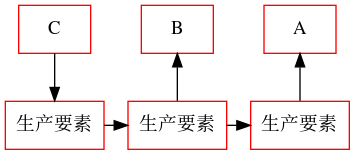
\includegraphics[scale=0.8]{weisebianji.png}
  \caption{\label{fig:weise}价值因果关系}
\end{figure}

边际效用经济学家认为,古典经济学家在声称价格取决于生产成本时是错误
的。\cref{fig:weise}揭示了这一所谓误解的准确性质。如果我们只考虑边际内产品,或者
肤浅地着眼于价格的形成,那么因果关系似乎就是从生产要素到价格——要素是决定价格的
因素。然而,根据边际效用经济学家的观点,仔细考虑这一过程就会发现,用来度量生产要
素价格的是生产要素在所生产的边际(或者说最后的最终产品,本例即胡萝卜(C))中产生的边际效
用。

\subsection{欧根·冯·庞巴维克}

庞巴维克与维色年龄相同;两人都是门格尔的学生,他们是朋友也是连襟。维色主要在奥地
利和德国有影响力,而庞巴维克在英国和美国更加为人所知。在庞巴维克的第一本书出版之
后,他在英国收了一个弟子,名叫威廉·斯马特(William Smart),他翻译了庞巴维克1890年
的《资本与利息》和1891年的《资本实证论》。门格尔在说英语的国家影响较小的一个原因
是,他的《原理》直到1950年才被翻译成英文出版。庞巴维克是一位造诣深厚的学者,他在
资本与利息领域的著作出版了三卷。第一卷《资本与利息:经济理论的批判史》涉及了远至
希腊的150多位经济学家。他花了大约二十年的时间来完成这套三卷本著作,在这期间的大部
分时间里,他是奥地利政府的重要人物。他对经济学的贡献,包括他对门格尔边际效用观点
的清晰说明与扩充,以及对资本与利息理论的发展(我们将在第9章中予以探讨)。像他的老师
门格尔以及他的同事和朋友维色一样,庞巴维克也没有运用数学。他运用推理的单因果关系
线条,详细说明关于价值或价格形成的观点,但他没有看出瓦尔拉斯和马歇尔所指出的相互
决定关系,这种关系现已成为现代经济思想的一个重要构件。

\subsection{走哪一条路——变化中的经济学范围与方法}

杰文斯、门格尔还有瓦尔拉斯,对现代经济学的技术工具做出了重大贡献,他们对于后来经
济思想的范围与方法也具有深远的影响。

三位经济学家都格外关注资源配置,或者被称作微观经济理论的东西。考虑到门格尔,我们
必须对这一宽泛的陈述进行限定,他在其《原理》第5部分考察了知识在人类福利进步中的作
用和影响。门格尔希望这样做能够补充和完善亚当·斯密对劳动分工的强调,即把劳动分工视
为国民福利提高的主要原因。不幸的是,门格尔的见解,即知识的作用是经济增长与发展的
因素,并没有被下一代的经济学家继续予以研究,他们变得几乎专门对资源配置感兴趣。
在1870--1900年期间,经济学从涉及斯密、李嘉图、穆勒的问题,转向研究价格系统如何运
行来分配稀缺资源。

尽管关于经济学的适当范围,杰文斯、门格尔、瓦尔拉斯之间具有几乎完全的一致性,然而,
关于适当的方法,他们的观点还是有分歧的。杰文斯追随威廉·配第的路线,提倡更多地运
用统计过程来确定经济变量之间的因果关系。门格尔偏重于更多地运用抽象推理,通过演绎
逻辑的使用构建学术模型。在这点上,他沿袭了李嘉图的方法。门格尔的研究缺乏数学、统
计学以及对历史过程或制度安排的论述。瓦尔拉斯的方法同样也缺少对时间或地点的抽象,
但是他确信,通过运用数学,能够了解市场经济的相关性和相互的因果关系。

经济学主流主要沿着两条道路前进:其一是更多地运用数学形式的抽象推理,即瓦尔拉斯所
建议的道路;另一个是更多地强调运用统计过程检验理论假设,即杰文斯所建议的道路。在
本书第四部分“现代经济学及其批判”中,我们将转向这类问题。

\subsection{杰文斯、门格尔以及瓦尔拉斯对后来经济学家的影响}

杰文斯从未有过追随者,所以,不存在杰文斯经济思想流派。马歇尔对英国经济思想的支配,
室息了杰文斯的贡献。杰文斯46岁时在一次游泳事故中过时离世,这也是他缺少追随者的原
因。瓦尔拉斯对边际分析的贡献,完全因其对一般均衡的阐述而失色。门格尔对经济学家和
经济学后来发展的影响,仍然在继续中。受到门格尔影响的相当多的经济学家在德国、英国
以及美国从事教学和研究;较早的一群人中包括米塞斯和熊彼特,较近的一群人中包括弗里
德里希·冯·哈耶克(1899--1992)、戈特弗里德·哈伯勒(1900--1995)以及奥斯卡·摩根斯
特恩(OskarMorgenstern,1902--1977)。在这些经济学家中,有些人独自研究,在任何重
要的方面都没有遵循奥地利传统,但有些人的确符合某种模式,我们能够描绘出从门格尔开
始,经维色、庞巴维克、米塞斯、哈耶克,到20世纪末奥地利经济学的世系。门格尔所提倡
的方法并没有为主流经济思想家所接受,他们更多地使用包含数学和统计学的方法。然而,
奥地利传统足以引起注意,所以,我们将在第13章中予以论述,并在第17章详细考察其现代
拥护者,那一章包含了一些现代非主流经济思想。

在受到门格尔影响的人中,很多都是市场驱动型经济体的拥护者,他们不满于社会主义者提
供的可替代选择。米塞斯和哈耶克在20世纪20年代开始的辩论中扮演了重要的角色,这些辩
论涉及:(1)社会主义经济体有效配置资源的能力,(2)资本主义、社会主义、经济与政治自
由三者之间的关系。我们在第13童中将转向这些问题,考察从事资本主义和社会主义研究的
奥地利经济学家及其他经济学家。

\section{总结}

凭借对边际分析的贡献,杰文斯、门格尔还有瓦尔拉斯,开创了新古典经济学。杰文斯和门
格尔认为,他们用需求导向的边际效用价值理论,替代供给导向的生产成本价值理论,对经
济理论进行着革命。然而,他们的希望没能得到实现,原因在于,他们专门强调需求方面,
同古典学者强调供给方面一样不完善。事实上,关于价值问题,杰文斯的和门格尔的看法从
根本上说是不合理的,因为他们在寻找边际效用与价格之间简单的因果关系。当古典经济学
家本质上假定需求既定,从而推断供给决定价格时,杰文斯和门格尔则假定供给既定,并推
断需求决定价格。瓦尔拉斯对价值问题有更加清晰的理解,因为他认识到经济体组成部分的
相互依赖。

三位经济学家对经济理论做出了五个永久性的贡献。(1)他们对边际效用和需求作用的强调,
促使后来的经济学家更多地注意价值理论中的这一部分内容。(2)他们对边际分析的运用,
导致人们对更普遍地使用这一方法的公认,这种公认对经济理论的发展产生了重要后果。
到1890年,边际分析已经被扩展到不仅涵盖家庭需求方面和厂商供给方面,而且包括厂商对
生产要素的需求方面。(3)杰文斯和瓦尔拉斯在经济理论化过程中对数学的应用,使经济学
家了解了这种分析类型的能力,并最终导致如今数学模型在经济思想中占支配地位。(4)就
提供市场经济不同部门相关性的见解,以及为后来的理论工作提供基础而言,瓦尔拉斯的一
般均衡模型是开创性的。(5)杰文斯对统计学的运用和认可,对于用计量经济学方法进行理论
检验的出现来说,泵重要的一步。

然而,边际分析的传播并不是迅速的,关于这一新方法,引起了很多和争议。我们将在接下
来的三章中研究边际主义和新古典微观经济学的成长。


%%% Local Variables:
%%% mode: latex
%%% TeX-master: "../../main"
%%% End:
